% Example LaTeX document for GP111 - note % sign indicates a comment
\documentclass[12pt]{article}
\usepackage{amsmath}
\usepackage{amsfonts}
\usepackage{amssymb}
\usepackage{mathabx}
\usepackage{mathtools}
\usepackage{listings}
\usepackage{cite}
\usepackage{graphicx}
\usepackage[margin=4cm]{geometry}
\usepackage{fancybox}
\usepackage{color}

\definecolor{mygreen}{rgb}{0,0.6,0}
\definecolor{mygray}{rgb}{0.5,0.5,0.5}
\definecolor{mymauve}{rgb}{0.58,0,0.82}
\DeclarePairedDelimiter\floor{\lfloor}{\rfloor}

\lstset{ %
  backgroundcolor=\color{white},   % choose the background color; you must add \usepackage{color} or \usepackage{xcolor}
  basicstyle=\footnotesize,        % the size of the fonts that are used for the code
  breakatwhitespace=false,         % sets if automatic breaks should only happen at whitespace
  breaklines=true,                 % sets automatic line breaking
  captionpos=b,                    % sets the caption-position to bottom
  commentstyle=\color{mygreen},    % comment style
  deletekeywords={...},            % if you want to delete keywords from the given language
  escapeinside={\%*}{*)},          % if you want to add LaTeX within your code
  extendedchars=true,              % lets you use non-ASCII characters; for 8-bits encodings only, does not work with UTF-8
  frame=single,                    % adds a frame around the code
  keepspaces=true,                 % keeps spaces in text, useful for keeping indentation of code (possibly needs columns=flexible)
  keywordstyle=\color{blue},       % keyword style
  language=Octave,                 % the language of the code
  morekeywords={*,...},            % if you want to add more keywords to the set
  numbers=left,                    % where to put the line-numbers; possible values are (none, left, right)
  numbersep=5pt,                   % how far the line-numbers are from the code
  numberstyle=\tiny\color{mygray}, % the style that is used for the line-numbers
  rulecolor=\color{black},         % if not set, the frame-color may be changed on line-breaks within not-black text (e.g. comments (green here))
  showspaces=false,                % show spaces everywhere adding particular underscores; it overrides 'showstringspaces'
  showstringspaces=false,          % underline spaces within strings only
  showtabs=false,                  % show tabs within strings adding particular underscores
  stepnumber=2,                    % the step between two line-numbers. If it's 1, each line will be numbered
  stringstyle=\color{mymauve},     % string literal style
  tabsize=2,                       % sets default tabsize to 2 spaces
  title=\lstname                   % show the filename of files included with \lstinputlisting; also try caption instead of title
}
% Default margins are too wide all the way around.  I reset them here
\setlength{\topmargin}{-.5in}
\setlength{\textheight}{9in}
\setlength{\oddsidemargin}{.125in}
\setlength{\textwidth}{6.25in}
\begin{document}
\title{Desarrollo e implementaci\'{o}n de c\'{o}digos polinomiales para la
detecci\'{o}n de errores en sistemas digitales (CRC$_{k}$).}
\author{Sebasti\'{a}n Valencia Calder\'{o}n\\
Juan Camilo Bages \\
Universidad de los Andes}
\renewcommand{\today}{Abril 11, 2014}
\maketitle
El siguiente informe, documenta el proceso de an\'{a}lisis y desarrollo de
algoritmos de detecci\'{o}n de errores en la transmisi\'{o}n para datos en redes
digitales. Sin embargo, la implementaci\'{o}n no se desarrolla en el \'{a}mbito
de las redes de comunicaci\'{o}n, sino, m\'{a}s bien, en un marco general
para entender el funcionamiento y utilidad de los algoritmos de detecci\'{o}n de
errores en problemas pr\'{a}cticos de ingenier\'{i}a. El proceso de
an\'{a}lisis, se realizar\'{a} usando pseudoc\'{o}digo (omitiendo detalles de
especificaci\'{o}n y an\'{a}lisis de eficiencia), mientras la implementaci\'{o}n
y desarrollo pr\'{a}ctico se realizar\'{a}n ambos usando el lenguaje de
programaci\'{o}n C. En concreto, el algoritmo que se analizar\'{a},
dise\~nar\'{a}, e implementar\'{a}, ser\'{a} CRC (Cyclic redundancy check, por
sus siglas en ingl\'{e}s), por sus facilidades de implementaci\'{o}n y
desarrollo. La t\'{e}cnica original, fue planteada y dise\~nada por Richard
Hamming. Est\'{a} t\'{e}cnica, es usada actualmente por la IEEE, para internet.

\section {Introducci\'{o}n}
En transmisi\'{o}n digital de datos, los erores ocurren cuado un bit es alterado
entre el proceso de transmisi\'{o}n y recepci\'{o}n; es decir, {\em0b1} es
transmitido mientras se recibe {\em0b0}, o viceversa. Adem\'{a}s de este tipo de
errores, la perdida de informaci\'{o}n puede ocurrir, lo que acarrea problemas a
la hora de la reconstrucci\'{o}n de la informaci\'{o}n, y de la comprensi\'{o}n
de la misma. Los errores pueden ser m\'{a}s graves que la p\'{e}rdida o
alteraci\'{o}n de un s\'{o}lo bit, p\'{e}rdidas o alteraciones m\'{a}s grandes
pueden ocurrir, es decir, una trama entera de datos, puede verse afectada, o
puede sufrir alteraciones importantes para la integridad de los datos.\\

La presencia de errores, es independiente al dise\~no del sistema de
transmisi\'{o}n, o del dise\~no de complejos protocolos de comunicaci\'{o}n. Por
lo tanto, es importante, preveer la presencia de errores y tratar de detectarlos
y en ocasiones corregirlos. Para este prop\'{o}sito, existen, ciertas
t\'{e}cnicas de detecii\'{o}n y correcci\'{o}n de errores sobre tramas de datos
transmitidas a trav\'{e}s de una red. Por pragmatismo, y eficiencia, se omiten
especificaciones de dise\~no y procesos de los algoritmos dise\~nados en el
largo desarrollo de las redes digitales, para compensar esto, la
bibliograf\'{i}a ofrece teor\'{i}a sobre el plantemiento te\'{o}rico de estos
procesos algoritmicos.

\section {Marco te\'{o}rico}

Una t\'{e}cnica com\'{u}n pero de todas maneras poderosa, de detecci\'{o}n de
errores es CRC (debe ser claro, que el objetivo general en el dise\~no de
algoritmos de detecci\'{o}n de errores, es maximizar la probabilidad de detectar
errores usando \'{u}nicamente un n\'{u}mero m\'{i}nimo de bits redundantes), el
cual se basa sobre un \'{a}rea poderosa de las matem\'{a}ticas para lograr
\'{e}ste objetivo. Los fundamentos te\'{o}ricos de \'{e}sta t\'{e}cnica es la
teor\'{i}a de campos algebr\'{a}icos. CRC, a veces se refiere como una
t\'{e}cnica de c\'{o}digos polinomiales, debido a la posibilidad de
representaci\'{o}n de tramas de bits usando polinomios. En general, un mensaje
de $(n + 1)$-bit, puede representarse usando un polinomio de grado $n$,
 usando como coeficiente de c\'{a}da t\'{e}rmino, el bit correspondiente por
posici\'{o}n en el mensaje total. Por ejemplo, para el mensaje de 8-bit
{\em0b10011010}, existe un polinomio representativo $M(x)$ donde $M(x) = 1
\times x^7 + 0 \times x^6 + 0 \times x^5 + 1 \times x^4 + 1 \times x^3 + 0
\times x^2 + 1 \times x^1 + 0 \times x^0 = x^7 + x^4 + x^3 + x^1$. Por lo tanto,
el proceso de transmisi\'{o}n puede entenderse como un proceso de intercambio de
polinomios.\\

Hasta ahora, nada se ha dicho sobre la naturaleza computacional del CRC, sino,
se han explicado las bondades de la correcci\'{o}n y detecci\'{o}n de
errores en datos. Antes de proceder con una definici\'{o}n y descripci\'{o}n
meramente formal de la derivaci\'{o}n de los c\'{o}digos de redundancia c\'{i}clica, se da una
descripci\'{o}n informal y general de la naturaleza del algoritmo. Un
matem\'{a}tico, entiende CRC como la computaci\'{o}n del residuo de la
divisi\'{o}n de dos polinomios con coeficientes en $\mathbb{Z}_{2}$. Un
cient\'{i}fico de la computaci\'{o}n, comprende CRC como la computaci\'{o}n del
residuo de la divisi\'{o}n de dos n\'{u}meros binarios, uno representando el
mensaje, y otro, un divisor fijo. Para los cript\'{o}grafos, CRC, es la
computaci\'{o}n de una operaci\'{o}n matem\'{a}tica sobre el campo de Galois de
orden 2 ($\mathbb{GF}_{2}$). Para los programadores, CRC, es el proceso que
itera sobre un mensaje y usa una tabla para obtener valores aditivos para cada
paso de la iteraci\'{o}n. Para los ingenieros y arquitectos de Hardware, CRC, es
el resultado computacional del proceso de un circuito l\'{o}gico que usa
divisi\'{o}n y repetici\'{o}n.\\

La descripci\'{o}n anterior, sugiere que CRC, es una t\'{e}cnica basada en
poderosas matem\'{a}ticas, es \'{u}til para cualquier longitud de mensaje, es un
proceso compacto, con una f\'{a}cil implementaci\'{o}n en hardware, y por lo
tanto en software (siempre y cuando se use un lenguaje con facilidades de
manejo de bajo nivel.\\

\begin{figure}
\centering
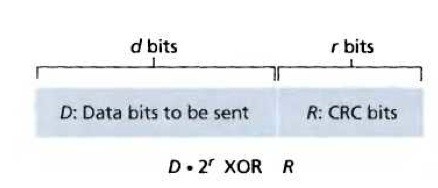
\includegraphics[width=90mm]{img1.jpg}
\caption{Mensaje enviado con la trama de redundancia}
\label{overflow}
\end{figure}

Para formalizar el proceso, consid\'{e}rese que el transmisor y receptor, deben
que ponerse de acuerdo en la elecci\'{o}n de un polinomio divisor $C(x) \in
\mathbb{P}_{k}$. Cuado el transmisor desea enviar o transmitir un mensaje
$M(x)$ de $n + 1$ bits, lo que se env\'{i}a realmente es el mensaje de $(n +
1)$-bit mas $k$ bits de redundancia para la posterior verificaci\'{o}n del
mensaje por parte del receptor. El mensaje completo, incluyendo los bits de reduncdancia es
$P(x)$. Las matem\'{a}ticas b\'{a}sicas, ayudan a inferir que $P(x)$ es
divisible por $C(x)$. Si $P(x)$ es transmitido a trav\'{e}s de un canal y no hay
errores en la transmisi\'{o}n, el receptor al dividir $P(x)$ por $C(x)$, debe
obtener cero. De lo contrario, sabemos que ha ocurrido un error. Para entender
mejor el proceso, es mejor entender un poco de aritm\'{e}tica binaria, lo cual
facilitar\'{a} la futura implementaci\'{o}n en C. La figura 1, muestra el
mensaje transmitido con la redundancia incluida (tomado de Kurose \& Ross, ver
bibliografi\'{i}a).\\

Al lidiar con n\'{u}meros en $\mathbb{Z}_{2}$, la aritm\'{e}tica, se simplifica
al usar operaciones modulo 2. Para resumir los vericuetos te\'{o}ricos, se
resumen las propiedades de est\'{a} aritm\'{e}tica a trav\'{e}s de polinomios.
Para considerar esto, considerese una funci\'{o}n $G : \mathbb{P}_{k}
\rightarrow \mathbb{Z}$, cuya descripci\'{o}n o especificaci\'{o}n es tomar un
polinomio y devolver su grado, o mayor potencia de la variable de
evaluaci\'{o}n.

\begin{itemize}
  \item $B(x) \mid C(x) \iff G(B) \geq G(C)$
  \item $B(x) \bmod C(x) = B(x) \oplus C(x)$
\end{itemize}

Una vez dispuestas estas reglas, es posible realizar divisi\'{o}n de tramas de
bits. Si se quiere transmitir o crear un polinomio para la transmisi\'{o}n
derivado del mensaje original $M(x)$, que sea $k$ bits m\'{a}s largo que $M(x)$,
y sea divisible por $C(x)$, se puede realizar el siguiente proceso: \\

\begin{itemize}
  \item $M(x) \times x^k$, es agregar $k$ ceros al final del mensaje
  \item $R(x) = T(x) \bmod C(x)$
  \item $T(x) - R(x)$
\end{itemize}

Al final es f\'{a}cil ver que el mensaje resultante es $M(x)$, seguido por el
residuo obtenido en el paso 2. Como ejemplo, consideremos el mensaje $10011010$,
y el c\'{o}digo es $CRC_{3} = 1101$. Primero, multiplicamos el polinomio
caracter\'{i}stico del CRC, obtenemos $10011010000$. Ahora se divide esto por
$C(x) = 1101$. El proceso de muestra en la figura 2 (tomado de Peterson \&
Davie). N\'{o}tese que el proceso es la utilizaci\'{o}n consecutiva de la
operaci\'{o}n XOR. Finalmente, el mensaje transmitido es $10011010101$, donde
los tres \'{u}ltimos d\'{i}gitos son correspondientes al residuo.

\begin{figure}
\centering
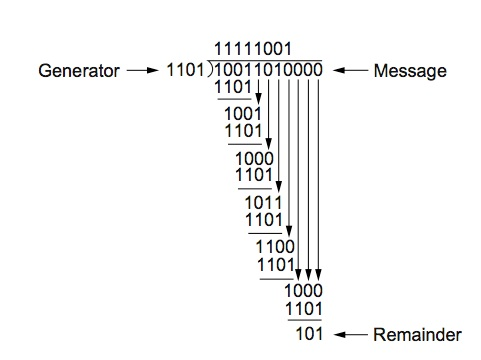
\includegraphics[width=90mm]{img2.jpg}
\caption{Calculo de CRC, usando divisi\'{o}n polinomial}
\label{overflow}
\end{figure}

A continuaci\'{o}n se muestra una table con los polinomios m\'{a}s comunes en la
pr\'{a}ctica.

\begin{center}
\begin{tabular}{ |l|l| }
  \hline
  \multicolumn{2}{|c|}{CRC m\'{a}s usados en la pr\'{a}ctica} \\
  \hline
  $CRC_{8}$ & $x^8 + x^2 + x^1 + 1$ \\
  $CRC_{10}$ & $x^10 + x^9 + x^5 + x^4 + x^1 + 1$ \\
  $CRC_{12}$ & $x^12 + x^11 + x^3 + x^2 + x + 1$ \\
  $CRC_{16}$ & $x^16 + x^15 + x^2 + 1$ \\
  $CRC_{16'}$ & $x^16 + x^12 + x^5 + 1$ \\
  $CRC_{32}$ & $x^32 + x^26 + x^23 + x^22 + x^16 + x^12 + x^11 + x^10 + x^8 +
  x^7 + x^5 + x^5 + x^2 + x + 1$ \\
  \hline
\end{tabular}
\end{center}

\section {Desarrollo}

Para asistir el proceso de depuraci\'{o}n, se presenta un procedimiento para
imprimir una entidad sin signo (unsigned), dado el valor, y la cantidad de bits
usabas para la representaci\'{o}n. Es decir, si se llama
binaryRepresentation(36, 16), esto debe imprimir $0000000000100100$. En la
siguiente p\'{a}gina se muestra el c\'{o}digo. Para el desarrollo de la
funci\'{o}n $darTamanho() : \mathbb{U} \rightarrow \mathbb{Z}$, se razon\'{o} de
la siguiente manera. La especificaci\'{o}n del procedimiento es calcular el
n\'{u}mero de bits necesarios para representar un n\'{u}mero decimal en el
sistema binario.\\

\textbf{Teorema}: El n\'{u}mero de bits necesarios para representar $n \in
\mathbb{Z}$ en $\mathbb{Z}_{2}$ est\'{a} dado por $\floor{\log_{2} n} + 1$. \\

\textbf{Demostraci\'{o}n} :
Sea $m$ el n\'{u}mero de bits necesarios para rpresentar $n \in \mathbb{Z}$,
esto es:
$$n = b_{m-1} \times 2^{m-1} + b_{m-2} \times 2^{m-2} + \ldots + b_{1} \times
2 + b_{0}$$

$$n = \sum_{i = 0}^{m - 1} b_i \times 2 ^{i} \mid b_{m-1} = 1 \wedge b_{i} \in
\mathbb{Z}_{2} \wedge i \in [0, m - 1)$$

$$n \leq \sum_{i = 0}^{m - 1} 2 ^{i} = 2^{m} - 1 < 2^m$$
$$\log_{2} n < m$$

Dado que $b_{m-1} = 1$, tenemos una cota inferior para n, es decir, $n \geq
2^{m-1}$ y por lo tanto, $\log_{2} n \geq m - 1$, dado que $m \in \mathbb_{Z}$,
$m - 1 = \floor{\log_{2} n}$, despejando tenemos que, $m = \floor{\log_{2}
n} + 1$. Esto se considera una prueba formal de que darTamanho(unsigned short
arg), puede escribirse como $floor(log2(arg)) + 1$.\\



\lstdefinestyle{customc}{
  belowcaptionskip=1\baselineskip,
  breaklines=true,
  frame=L,
  xleftmargin=\parindent,
  language=C,
  showstringspaces=false,
  basicstyle=\footnotesize\ttfamily,
  keywordstyle=\bfseries\color{green!40!black},
  commentstyle=\itshape\color{purple!40!black},
  identifierstyle=\color{blue},
  stringstyle=\color{orange},
}

\lstset{escapechar=@,style=customc}

\begin{lstlisting}
void binaryRepresentation(unsigned number, int bits) {
	int need = darTamanho(number), counter;
	char array[bits];
	for(counter = 0; counter < bits; counter++)
		array[counter] = '0';
	counter = bits - 1;
	while(number != 0) {
		int flag = number % 2;
		array[counter] = (flag == 1)? '1' : '0';
		counter--;
		number = number / 2;
	}
	for(counter = 0; counter < bits; counter++)
		printf("%c", array[counter]);
	printf("\n");
}
\end{lstlisting}

Para el desarrolo de la funcci\'{o}n ``unsigned short leerPrimerBloque(TEXTO
*datos)'', esta se especifica como la que extrae los dos primeros bytes para
conformar un short, para esto, se ingresa por valor al mensaje de la estructura,
a su tama\~no, y se corre un n\'{u}mero binario, las posiciones necesarias para
llenar un short. El proceso est\'{a} expl\'{i}cito en el c\'{o}digo. Para la
funci\'{o}n ``void corregirPrimerBloque(unsigned short * primerBloque)'', se
extraen los bits desde la posici\'{o}n m\'{a}s significativa hasta completar el
tama\~no de $k$, para esto, consid\'{e}rese el siguiente procedimiento, cuyo
objetivo es extraer los $n$- bit de x desde p hacia atr\'{a}s, asumiendo que
la posici\'{o}n menos significativa es la 0, y que $p, n \in \mathbb_{Z}$.
Entonces, $getbits(x, 4, 3)$, retorna los bits en la posici\'{o}n 4, 3 y 2.:\\

\begin{lstlisting}
unsigned getbits(unsigned x, int p, int n) {
	return (x >> (p+1-n)) & ~(~0 << n);
}
\end{lstlisting}

En el anterior procedimeinto, la expresi\'{o}n $(x >> (p+1-n))$, mueve el campo
deseado a la derecha de la palabra. $~0$ es $1111 \ldots 1111$, mover a la
izquierda n bit con la expresi\'{o}n $~(~0 << n)$, acomoda ceros en las $n$ 
posiciones menos significativas. Complementando con $~$, permite devolver los
$n$ bit m\'{a}s a la derecha. Siuiendo este razonamiento, puede decirse que dado
el primer bloque, es necesario obtener desde la posici\'{o}n m\'{a}s
significativa hasta k del primer bloque.\\

Para reemplazar ceros, descrita a continuaci\'{o}n, se toma unos Bytes de solo
unos y se corre $k - 1$, tal y como se desea, se toma en AND con el residuo, y
esto se guarda en la variable shift, luego, se cambia el valor del mensaje por
su valor actual OR lo que se hab\'{i}a calculado antes.\\

\begin{lstlisting}
void reemplazarCeros(TEXTO * txt, unsigned short residuo) {
	unsigned short shift = residuo & ~(~0 << k - 1);
	*txt->mensaje = *txt->mensaje | shift;
}
\end{lstlisting}

Para agregar bit, la funci\'{o}n que agrega el bit que llega por par\'{a}metro
a txt, se debe entender el bit que llega, es decir pasar de char a int, y luego
se agrega por valor. Para esto, se corre *txt al lado del bit m\'{a}s
significativo y se hace OR con el bit que llega, pues si es cero, para el
computador es $0000 \ldots 0000$, si es uno, para el computador es $000 \ldots
0001$.\\

\begin{lstlisting}
void agregarBit(unsigned short * txt, unsigned char bit) {
	int realBit = (bit == '0')? 0 : 1;
	*txt = (*txt << 1) | realBit;
}
\end{lstlisting}

El razonamiento para ``unsigned char bajarDigito(unsigned char * msj, int
bitpos)'', es similar, pues se debe reconocer el bit, que representa la
posici\'{o}n, y posteriormente devolver el bit en esta posici\'{o}n. Lo que debe
hacer esta funci\'{o}n es devolver el d\'{i}gito en la posici\'{o}n que llega
por par\'{a}metro. Para su desarrollo, se us\'{o} el razonamiento expueso en
getbit.

\begin{lstlisting}
unsigned char bajarDigito(unsigned char * msj, int bitpos) {
	// (*msj >> bitpos) & 1
	int flag = (*msj >> bitpos) & ~(~0 << 1);
	return (flag == 0) ? '0' : '1';
}
\end{lstlisting}

\pagebreak

La estructura de las funciones hasta ahora definidas, se observan en el
siguiente c\'{o}digo, los detalles, est\'{a}n el el c\'{o}digo real.\\

\begin{lstlisting}
#include <stdio.h>
#include <stdio.h>
#include <stdbool.h>
#include <math.h>
#include <assert.h>

int k;

typedef struct text {
	unsigned char *mensaje;
	int tamanho;
} TEXTO;

int darTamanho(unsigned short bloq) {
	return floor(log2(bloq)) + 1;
}

void corregirPrimerBloque(unsigned short * primerBloque) {
	int tamanioMax = darTamanho(*primerBloque);
	int tamanioMin = k;	
	int p = tamanioMax - 1;
	int n = tamanioMin;
	*primerBloque = (*primerBloque >> (p + 1 - n) & ~(~0 << n));
}

void agregarBit(unsigned short * txt, unsigned char bit) {
	int realBit = (bit == '0')? 0 : 1;
	*txt = (*txt << 1) | realBit;
}

void reemplazarCeros(TEXTO * txt, unsigned short residuo) {
	unsigned short val = residuo & ~(~0 << (k - 1));
	* txt -> mensaje = * txt -> mensaje | val;
}

unsigned short leerPrimerBloque(TEXTO *datos) {
	int sizeOfMensaje = darTamanho(*datos->mensaje);
	unsigned short val = *datos->mensaje & (~0 << (sizeOfMensaje - 16));
	return val;
}

unsigned char bajarDigito(unsigned char * msj, int bitpos) {
	int flag = (*msj >> bitpos) & ~(~0 << 1);
	return (flag == 0)? '0' : '1';
}

void binaryRepresentation(unsigned number, int bits) {
	int need = darTamanho(number);
	assert(need <= bits);
	int counter;
	char array[bits];
	for(counter = 0; counter < bits; counter++)
		array[counter] = '0';
	counter = bits - 1;
	while(number != 0) {
		int flag = number % 2;
		array[counter] = (flag == 1)? '1' : '0';
		counter--;
		number = number / 2;
	}
	for(counter = 0; counter < bits; counter++)
		printf("%c", array[counter]);
	printf("\n");
}

int main(int argc, char const *argv[]) {
	int machine = 16;
	int generador = 350;
	k = darTamanho(generador);
	printf("%d\n", darTamanho(350));
	return 0;
}
\end{lstlisting}

Finalmente, para la divisi\'{o}n, se realiza el proceso tal y como se explica
en la gu\'{i}a, es decir, primero, se obtiene el bit en la posici\'{o}n actual
usando las funciones previamente definidas, posteriormente, se agrega al final
del residuo, y se repite hasta alcanzar el tama�o de k, en cuyo caso, se retorna
agregan los bits del residuo en la cola del mensaje.\\

\begin{lstlisting}
unsigned short division(TEXTO * txt, unsigned short generador)
{	
	unsigned short primerBloque=leerPrimerBloque(txt); 
	int tamanhoResiduo = darTamanho(primerBloque); 
	int posActual = 16; 
	unsigned short residuo;  
	unsigned char bitBajar;  
	int fin = ((txt->tamanho - 2) * 8) + (k - 1); 
	if (k<tamanhoResiduo) {
		corregirPrimerBloque(&primerBloque, k);
		posActual = 16-(tamanhoResiduo - k);
	}

	residuo = primerBloque;
	while (posActual < fin)
	{
		if (tamanhoResiduo < k)
		{
			unsigned char bitPosActual = bajarDigito((txt->mensaje), posActual);
			agregarBit(&residuo, bitPosActual);
			posActual++;
		}
		tamanhoResiduo = darTamanho(residuo);
		if(tamanhoResiduo == k) 
			reemplazarCeros(txt, residuo);		
	}
	return residuo;
}
\end{lstlisting}

\begin{thebibliography}{9}

\bibitem{lamport94}
  Larry L. Peterson,
  \emph{Computer Networks: A Systems Approach}.
  Elsevier Computers, Massachusetts,
  5th Edition,
  2011.
\bibitem{lamport94}
  James F. Kurose,
  \emph{Computer Networking: A Top-down Approach}.
  Pearson,
  6th Edition,
  2013.
\bibitem{lamport94}
  William Stallings,
  \emph{Data and Computer Communications}.
  Pearson Education,
  8th Edition,
  2007.
\bibitem{lamport94}
  Behrouz A. Forouzan,
  \emph{Data Communications and Networking}.
  Huga Media,
  4th Edition,
  2007.
 \bibitem{lamport94}
  Douglas Comer,
  \emph{Computer Networks and Internets: With Internet Applications}.
  Pearson/Prentice Hall,
  5th Edition,
  2004.
 \bibitem{lamport94}
  Andrew S. Tanenbaum,,
  \emph{Computer Networks: Pearson New International Edition}.
  Pearson Education, Limited,
  1st Edition,
  2013.
   \bibitem{lamport94}
  Peter J. Cameron,,
  \emph{Introduction to Algebra}.
  Oxford University press,
  2nd Edition,
  2008.
   \bibitem{lamport94}
  David S. Dummit,
  \emph{Abstract Algebra}.
  John Wiley and Sons. Inc,
  3rd Edition,
  2004.
   \bibitem{lamport94}
  Joseph A. Gallian,
  \emph{Contemporary abstract algebra}.
  Cengage learning,
  7th Edition,
  2010.
   \bibitem{lamport94}
  John G. Proakis,
  \emph{Communication systems engineering}.
  Prentice Hall,
  2nd Edition,
  2002.
   \bibitem{lamport94}
  Gilles Brassard,,
  \emph{Algorithmics: theory and practice}.
  Prentice Hall,,
  1st Edition,
  1988.
   \bibitem{lamport94}
  Brian W. Kernighan, Dennis Ritchie
  \emph{The C Programming Language}.
  Pearson Education,
  2nd Edition,
  1988.  
   \bibitem{lamport94}
  K. N King
  \emph{C Programming: A Modern Approach}.
  Granite Hill Publishers,
  2nd Edition,
  2010.
\end{thebibliography}

\end{document}
